\documentclass[11pt]{article}
\usepackage[utf8]{inputenc}

\usepackage{amssymb, amsmath, amsthm, amsfonts, algorithmic, algorithm, graphicx}
\usepackage{color}
\usepackage{bbm}
\usepackage[dvipsnames]{xcolor} 
\usepackage[colorlinks,linkcolor=blue,citecolor=blue]{hyperref}
\usepackage{array}
\usepackage{ifthen}
\usepackage{subfigure}
\renewcommand{\baselinestretch}{1.1}
\setlength{\topmargin}{-3pc}
\setlength{\textheight}{8.5in}
\setlength{\oddsidemargin}{0pc}
\setlength{\evensidemargin}{0pc}
\setlength{\textwidth}{6.5in}

\newtheorem{theorem}{Theorem}[section]
\newtheorem{lemma}[theorem]{Lemma}
\newtheorem{proposition}[theorem]{Proposition}
\newtheorem{corollary}[theorem]{Corollary}
\newtheorem{question}[theorem]{Question}
\newtheorem{result}[theorem]{Result}
\newtheorem{definition}[theorem]{Definition}
\newtheorem{example}[theorem]{Example}
\newtheorem{remark}[theorem]{Remark}
\newtheorem{assumption}[theorem]{Assumption}
\numberwithin{equation}{section}

\def \endprf{\hfill {\vrule height6pt width6pt depth0pt}\medskip}
\renewenvironment{proof}{\noindent {\bf Proof} }{\endprf\par}

% Notational convenience,
% real numbers 
\newcommand{\R}{\mathbb{R}}  
% Expectation operator
\DeclareMathOperator*{\E}{\mathbb{E}}
% Probability operator
\DeclareMathOperator*{\Prob}{\mathbb{P}}
\renewcommand{\Pr}{\Prob}

% You may define additional macros here.


\begin{document}

\begin{center}
    \sc Recurrent and Generative ANNs
\end{center}

\noindent Name: Bileam Scheuvens, Pankaj Bora

\noindent Email: benedictbileam@gmx.de, bora.pankajt1@gmail.com

\noindent Matr. Nr.:6983475, 6946375



\section{Exercise 1}
\subsection{(a)}
See code for implementation.
\newline
\subsection{(b)}

\subsubsection{LSTM}

\paragraph{Epoch 10:}

Initialization: ‘but the night will be too sho...

Tolkien: --- ‘but the night will be too short,’ said gandalf. ‘i have come back
here, for i must have a little peace, alone. you should sleep,

LSTM model: --- ‘but the night will be too shot te te te te te te te te te te te
te te te te te te te te te te te te te te te te te te te te te te

\paragraph{Observation:} Outputs repetitive meaningless sequences. LSTM hasn't yet learned to
model dependencies across time steps.

\paragraph{Epoch 100:}

Initialization: at last they came out of shado... Tolkien: --- at last they came
out of shadow to the seventh gate, and the warm sun that shone down beyond the
river, as frodo walked in the gla

LSTM model: --- at last they came out of shador and the store and the store of the
store and the store of the store and the store of the store and

\paragraph{Observation:} Can now capture basic word structures but still struggles with long
term dependencies, leading to repetition.

\paragraph{Epoch 482:}

Initialization: pippin gazed in growing wonder...

Tolkien: --- pippin gazed in growing wonder at the great stone city, vaster and
more splendid than anything that he had dreamed of; greater and

LSTM model: --- pippin gazed in growing wonder and stroke his head and seems that
is a have begone the many, and the lord of the shadow of the city

\paragraph{Observation:} Now outputs semantically plausible phrases. LSTM has learned to
capture dpendencies, and generates more coherent text. Mainly limited by it memory
horizon.

\subsubsection{TCN}

\paragraph{Epoch 10:}

Initialization: ‘then why did you not say so a...

Tolkien: --- ‘then why did you not say so at once?’ said bergil, and suddenly a
look of dismay came over his face. ‘do not tell me that he has

TCN model: --- ‘then why did you not say so
ayyyyyyyyyyyyyyyyyyyyyyyyyyyyyyyyyyyyyyyyyyyyyyyyyyyyyyyyyyyyyyyyyyyyyyyyyyyyyyyyyyyyyyyyyyyyyyyyyyyyy

\paragraph{Observation:} TCN fails to generalize patterns and latches onto most common tokens.

\paragraph{Epoch 100:}

Initialization: ‘man!’ cried pippin, now thoro... Tolkien: --- ‘man!’ cried
pippin, now thoroughly roused. ‘man! indeed not! i am a hobbit and no more valiant
than i am a man, save perhaps now

TCN model: --- ‘man!’ cried pippin, now thoro!!!

(((??

uu)))!!!

gggrrrrrrrrrrrrrrrrrrrrrrrrrrrrrrrrrrrrrrrrrrrrrrrrrrrrrrrrrrrrrrrrrrrrrrrrrr

\paragraph{Observation:} TCN's architecture unable to capture long term dependencies needed
for text generation leading to unstable and incoherent output.

\paragraph{Epoch 482}

Initialization: ‘that is good!’ said bergil. ‘...

Tolkien: --- ‘that is good!’ said bergil. ‘we boys are no longer allowed to pass
the gate without an elder. now we shall see better.’

TCN model: --- ‘that is good!’ said bergil. ‘j!u !! (followed by 100+ newlines)

\paragraph{Observation:} TCN overfits or collapses during training. Observing the loss, it
starts oscillating at around epoch 100 and never converges.

\subsubsection{Transformer}

\paragraph{Epoch 10:}

Initialization: ‘you are peregrin the halfling...

Tolkien: --- ‘you are peregrin the halfling?’ he said. ‘i am told that you have
been sworn to the service of the lord and of the city. welcome!

Transformer model: --- ‘you are peregrin the halfling the the the the the the the
the the the the the the the the the the the the the the t the the t the

\paragraph{Observation:} Struggles to capture sequence order, possibly due to lack of
positional embeddings.

\paragraph{Epoch 100:}

Initialization: pippin lifted it and presented...

Tolkien: --- pippin lifted it and presented the hilt to him. ‘whence came this?’
said denethor. ‘many, many years lie on it. surely this is a b

Transformer model: --- pippin lifted it and presented the hilt he him. ‘came the
seany,’ said inet lan ore our of the ling oredred in pan in the win the l

\paragraph{Observation:} Unable to effectively model dependencies between tokens in a
sequence, causing semantic errors. Still generates contextually relevant phrases.

\paragraph{Epoch 512:}

Initialization: ‘can you find your way?’ said ...

Tolkien: --- ‘can you find your way?’ said beregond at the door of the small hall,
on the north side of the citadel, where they had sat. ‘it is

Transformer model: --- ‘can you find your way?’ said beregond at the door of the
small hall, on the north side of the citadel, where they had sat. ‘it is

\paragraph{Observation:} Even without positional embedding, given that the training dataset is
limited, the model basically overfits to the training data, able to almost always
duplicate the original text.


\section*{Exercise 2}

\subsection{(a)}
See checkpoints for training results. 
VAE with $\beta =4$ was not trained as long as the others. For consistency we contrast only $\beta \in [0,20]$ but it can be reasonably assumed that $4$ would perform somewhere in between.
We unfortunately learned too late that we had to change the queue type from test to submit longer jobs, so we trained locally and were therefore slightly limited in our experiments.
\newpage
\subsection{(b)}

Images of a VAE with higher beta seem to have more contrast and look sharper but a
little less coherent/realistic, while the VAE with beta 0 produces blurry images
of plausible looking faces. Due to computational constraints it is likely that
neither model was trained to convergence, and it is thus unclear but likely that
this effect would persist or even amplify with more training. The beta value
enforces more distinct structure in the latent space, while a vanilla VAE is free
to learn an average of all possible faces.
Results can be seen in \ref{fig:samples}

\begin{figure}[h]
  \caption{16 Randomly sampled images with varying $\beta$}
  \label{fig:samples}
    \centering
    \begin{minipage}{0.4\textwidth}
        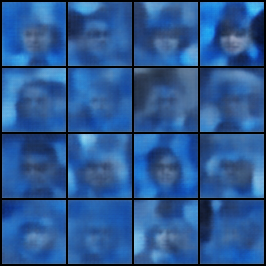
\includegraphics[width=\textwidth]{ex02/beta0.0-generated.png}
        \caption{$\beta =0$ }
    \end{minipage}
    \hspace{2cm}
    \begin{minipage}{0.4\textwidth}
        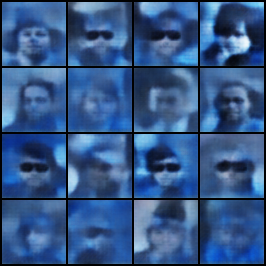
\includegraphics[width=\textwidth]{ex02/beta20.0-generated.png}
        \caption{$\beta =20$}
    \end{minipage}
\end{figure}

\newpage
\subsection{(c)}

For the vanilla VAE varying individual dimensions produces drastically different
faces, but it is rarely clear how to interpret this change as opposite faces have
little in common. Additionally many dimensions are similar in their output. For
the VAE with beta 20, the distinction is stronger and for many dimensions one can
make an educated guess about what the dimension represents, sunglasses vs hats
(dim 0 and 3), hair vs bald (dim 5) or skin color (dim 18).
Results can be seen in \ref{fig:variation}

\begin{figure}[h]
  \caption{Random latent vector with individually perturbed dimensions with varying $\beta$ }
  \label{fig:samples}
  \label{fig:variation}
    \centering
    \begin{minipage}{0.4\textwidth}
        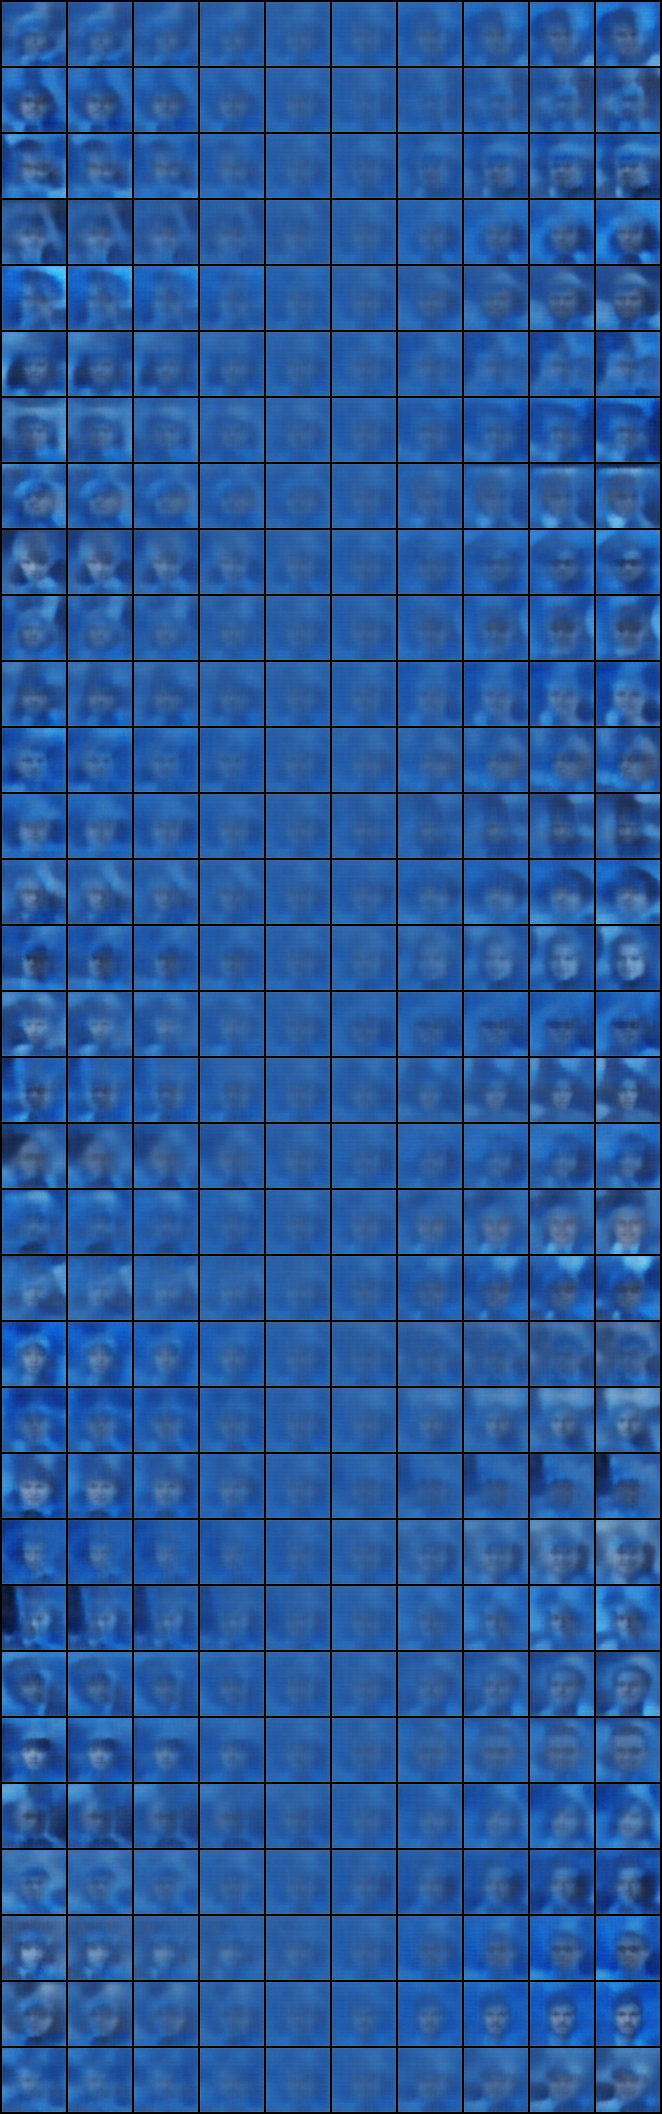
\includegraphics[width=\textwidth]{ex02/beta0.0-variation.png}
        \caption{$\beta = 0$}
    \end{minipage}
    \hspace{2cm}
    \begin{minipage}{0.4\textwidth}
        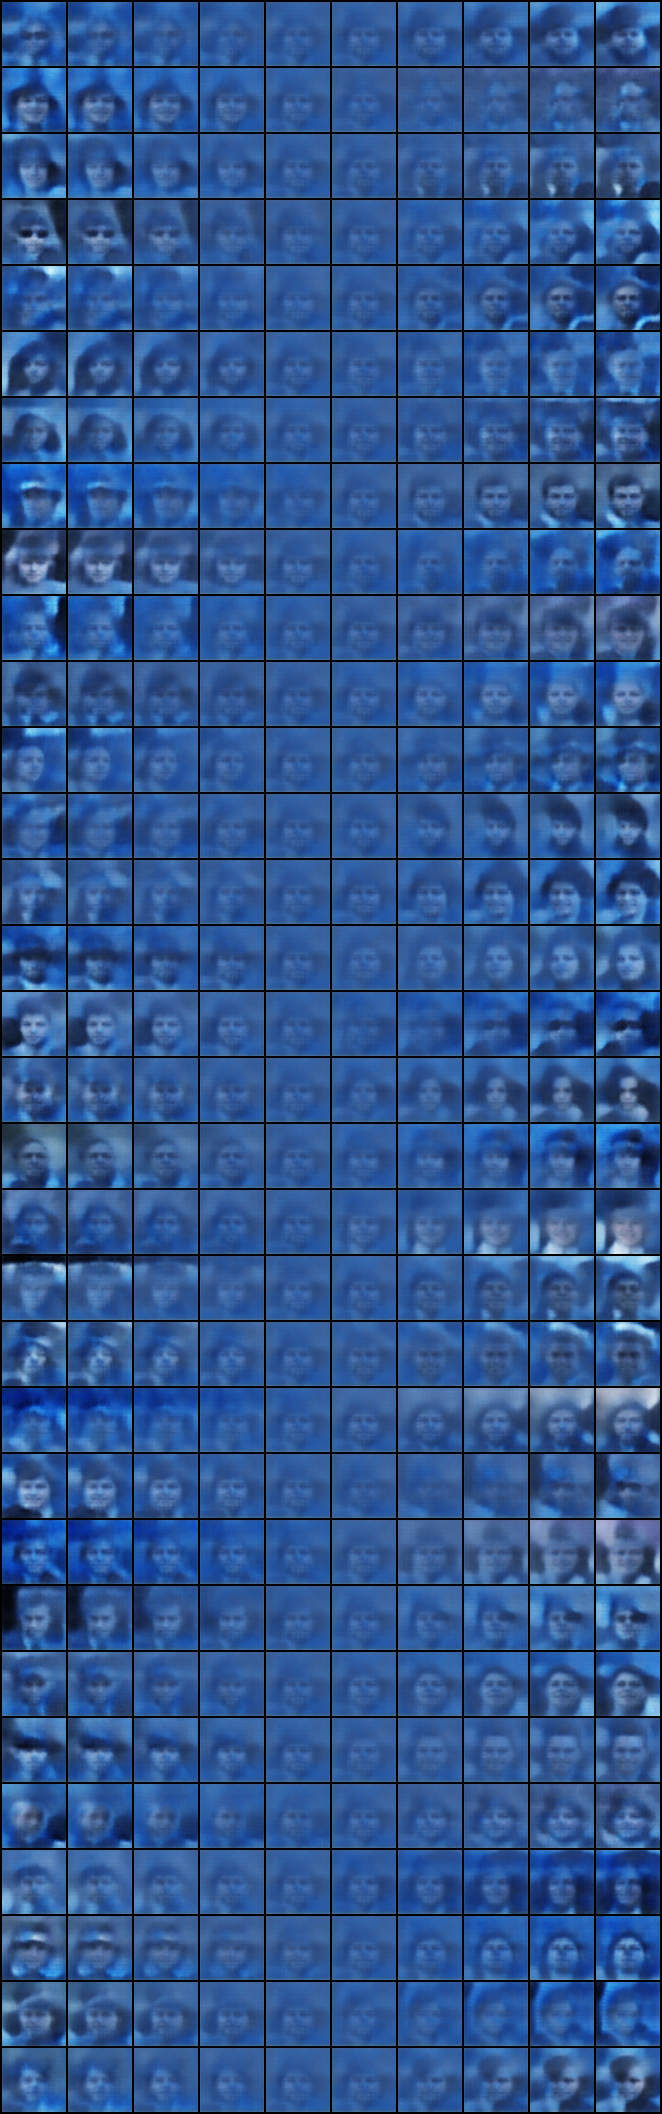
\includegraphics[width=\textwidth]{ex02/beta20.0-variation.png}
        \caption{$\beta =20$ }
    \end{minipage}
\end{figure}

\newpage
\subsection{(d)}

Multiple dimensions contain some information about rotation/ facial orientation,
but for our model, dimension 11 of the beta20 VAE was the most prominent. Still,
negative pertubations have little effect (possibly due to the sigmoid activation clamping the negative rotation away),
leaving the face mostly centered. Positive pertubations however rotate the face as
desired.
The face is not kept fully intact, in fact for drastic changes (like in the given example) the face is rotated correctly but barely resembles the original face.
Results can be seen in \ref{fig:rotation}.


\begin{figure}[h]
  \caption{Image rotated left and right (positive and negative latent dimension) }
  \label{fig:rotation}
  \label{fig:variation}
    \centering
    \begin{minipage}{0.4\textwidth}
        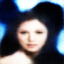
\includegraphics[width=\textwidth]{ex02/beta20.0-rotated_left.png}
        \caption{negative latent perturbation}
    \end{minipage}
    \hspace{2cm}
    \begin{minipage}{0.4\textwidth}
        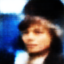
\includegraphics[width=\textwidth]{ex02/beta20.0-rotated_right.png}
        \caption{positive latent perturbation}
    \end{minipage}
\end{figure}
\end{document}
